\chapter{Introduction} \label{c:intro}

% http://ieeexplore.ieee.org/stamp/stamp.jsp?tp=&arnumber=6005328
% Instead, the image is dominated by speckle that is characteristic for coherent imaging. Speckle comes from the large variations in the intensity of backscattered radiation coming from the diversity in angles of the beam-target incidence, and it dominates any difference in the intrinsic reflectivity of, say, PVC pipe material, clothing, and skin.

%% RFI HSHQDC-14-00015
%% commercially available standoff - Brijot Gen 2, SET CounterBomber
%% TSA 700 AIT (advanced imaging technology) systems at 160 airports

For over thirty years the millimeter and submillimeter-wavelength spectrum has been the subject of instense interest for military and security maging applications.
The reason for this interest is that the spectral region from \SIrange{100}{1000}{\GHz} offers a good compromise between transmission through obscurant materials (favoring lower frequencies) and spatial resolution (favoring higher frequencies) \cite{kruse_why_1981}.
This interest has driven a long line of technological advancement in sources, detectors, and other technologies at these wavelengths \cite{popovic_thz_2011}.
This advancement has taken place in both ``active'' imaging, in which an observation target is illuminated by light and the reflections from that target are recorder, and `passive'' imaging, in which ambient thermal emissions are detected.

Over a similar timespan the same time the millimeter and sub-millimeter astronomical community has also been very interested in these wavelengths.
In particular, the desire to make more and more sensitive maps of the Cosmic Microwave Background (\CMB) radiation have driven this communities need for instruments capable of higher and higher sensitivies.
During the 1980's and early 1990's cooled bolometric detectors capable of achieving photon-noise-limited --- or near photon-noise-limited --- performance were developed.
By 1994 it was clear that for many astromonical applications the only way to increase sensitivity was to develop arrays of bolometers, but at that time no technology for the production of monolithic arrays was yet available \cite{richards_bolometers_1994}.

The development of voltage-biased superconducting Transition-Edge-Sensor detectors enabled the development of large-scale detector array.
These detectors are based on the use of thin superconducing films as the bolometer's themometry element, and can fabricated at large scale using standard lithographic techniques.
Their operation and advantages for array-scale operation are described in \chapterref{c:tes}.
To readout these detector arrays, several groups have developed \SQUID-based multiplexed readout systems.
This technology is now mature and is routinely deployed on both ground and balloon-borne experiements in arrays containing up to 10,000 bolometric detectors \cite{holland_scuba-2:_2013}.

The development of this technology offers new opportunities for passive imaging for security and other applications
Specifically, it is now possible to develop focal planes capable of video-rate imaging with temperature resolution of \SI{100}{\mK} or below.
This thesis decribes the design and development of the \NIST\ \Imager, a system developed to perform detection of concealed weapons at distances of \SIrange{26}{28}{\m} by producing video-rate images at \SI{350}{\GHz}.
This chapter provides an overview of millimeter-wavelength imageing and the problems that our system is intended to solve.

\section{Security Imaging}

The frequency range \SIrange{100}{1000}{\GHz} is attractive for detection of concealed weapons or contraband because many common clothing materials have hi transmission in this range \cite{bjarnason_millimeter-wave_2004}.
In general, as shown in \figref{fig:ch1-clothes-atmos-trans}, transmission through clothing steadily decreases as frequency inncreases.
This trend tends to push systems toward lower frequencies.
An example likely familiar to readers L3 Provision (correct name?) systems operating at many airports within the USA.
These are radar systems operating at ~\SI{35}{\GHz}, intended for close-range portal screening.
For applications in which is is acceptable to require individuals to pass through and pause at a particular location, these systems have excellent image quality.
Although the ProVision system only takes still images with a xxx s image acquisition time, similar portal screen systems with video-rate capabilities are also under development (xxx ref system from talk in Dresden).

\begin{figure*}
\centering
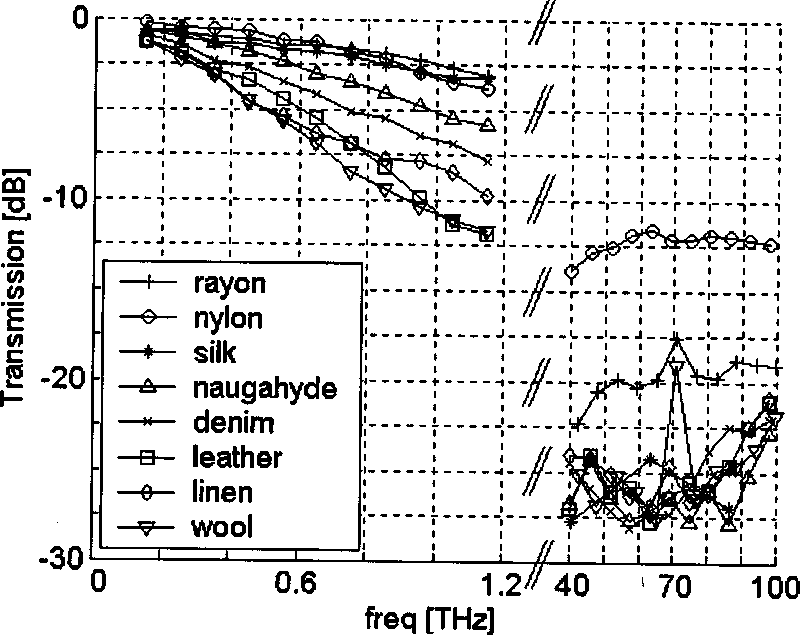
\includegraphics{drawings/ch1-clothes-bjarnason.pdf}
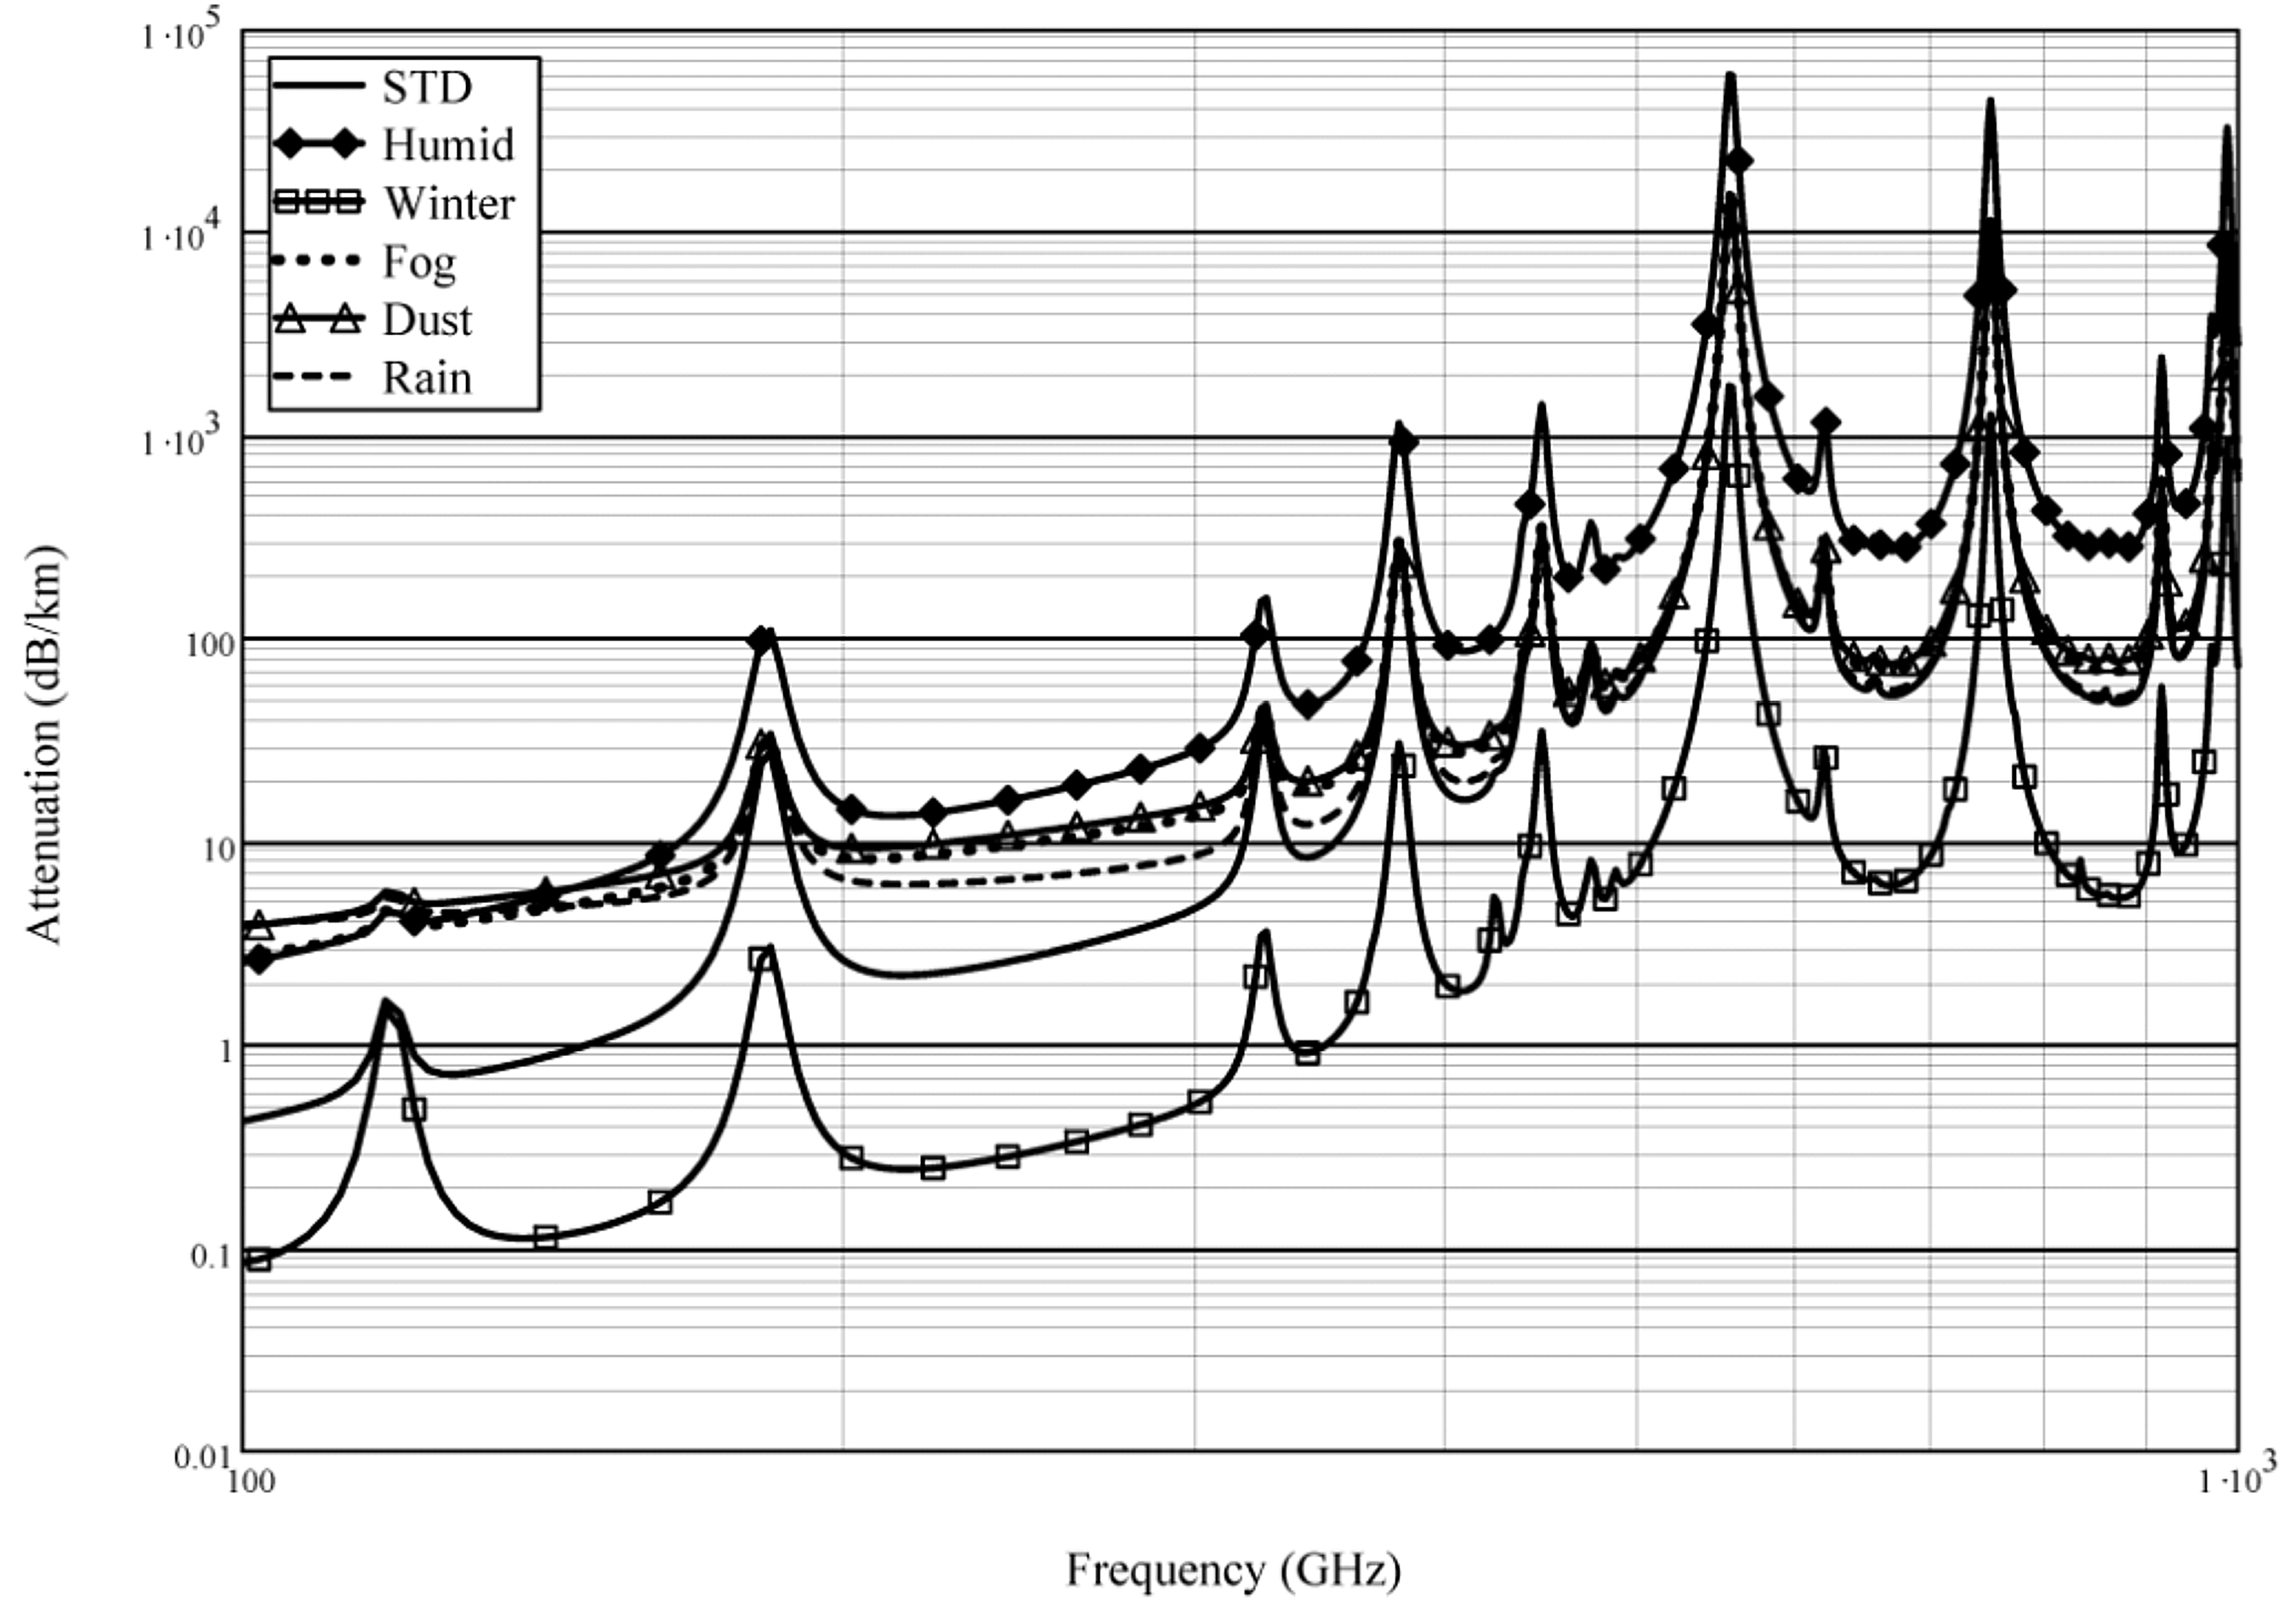
\includegraphics{drawings/ch1-atmos-trans.pdf}
\caption[Clothing and Atmospheric Transmission vs Frequency]{
  \textbf{Left}
  Plot of clothing transmission vs frequency.
  Taken from \cite{bjarnason_millimeter-wave_2004}.
  As frequency increases, transmission through all kinds of clothing decreases.
  The \SI{-10}{\dB} observation band of the \Imager\ is highlighted (\SIrange{318}{376}{\GHz}).
  \textbf{right}
  Plot showing a model of zenith atmospheric transmission on the summit of Mauna Kea, assuming \SI{0.5}{\mm} of percipital water vapor.
  The plot is illustrative only, demonstrating the presence of atmospheric transmission windows and the general trend of worse transmission at higher frequencies.
  The data was obtained using the Caltech Submillimeter Observatory (CSO) Atmospheric Transmission Interactive Plotter \cite{darek_lis_cso_????}, which is based on a published model \cite{pardo_atmospheric_2001}.
}
\label{fig:ch1-clothes-atmos-trans}
\end{figure*}

But there are other applications and operational screnarios in which portal screening system are not feasiable.
One example is detection of suicide bomb belts, a scenario in which is it desirable to make a detection while the person being observed is some distance away.
These applications are generally referred to as ``standoff'' detection because the imaging system ``stands off'' some distance from the target being imaged.

In addition, also as shown in \figref{clothes-atmos-trans}, atmospheric transmission also tends to decrease with frequency in this range, although there are many atmosheric and other windows present so that the increase is not monotonic.
One example is detection of suicide bomb belts.
